\documentclass[12pt, a4paper, oneside]{ctexart}
\usepackage{amsmath, amsthm, amssymb, appendix, bm, graphicx, hyperref, mathrsfs, graphicx}
\usepackage{authblk}
% \usepackage[perpage]{footmisc}
\usepackage{multirow}
\usepackage{hyperref}
\hypersetup{hidelinks,
	colorlinks=true,
	allcolors=black,
	pdfstartview=Fit,
	breaklinks=true}
\usepackage{float}
\usepackage{enumerate}

\linespread{1.5}

\renewcommand{\abstractname}{\Large\textbf{绪言}}
\newcounter{parnum}[section]
\newcommand{\N}{%
    \refstepcounter{parnum}%
    \makebox[0.7em][l]{\small{\arabic{parnum}}}
    }
% Use a generous paragraph indent so numbers can be fit inside the
% indentation space.
\setlength{\parindent}{2em}

\begin{document}

\setcounter{page}{0}
\begin{center}
	\Large{\textbf{马太福音}} \\ \vspace{2em}
	\small{\href{https://biblehub.com/bsb/matthew/}{Matthew}} \\ \vspace{1em}
	\small{译者：Job Zhao} \\ \vspace{1em}
	\small{编译日期: \today} \\ \vspace{1em}
	\small{Version 2.00} \\ \vspace{1em}
\end{center}
\vfill
\vspace{28em}
\begin{tabular*}{\textwidth}{cc}
	\includegraphics{figure/by-nc.eps}
	& \begin{minipage}[b]{0.6\textwidth}
		\footnotesize
		本作品采用知识共享署名-非商业性使用4.0国际许可协议进行许可。访问\url{http://creativecommons.org/licenses/by-nc/4.0/ }查看该许可协议。
	\end{minipage}
\end{tabular*}
\vspace{2mm}
\thispagestyle{empty}

\newpage

% \begin{abstract}
    
% \end{abstract}

\newpage
\pagenumbering{Roman}
\setcounter{page}{1}
\tableofcontents
\newpage
\setcounter{page}{1}
\pagenumbering{arabic}

% \section*{介绍}


\newpage

% Matthew 1
\section{第一章}

% The Genealogy of Jesus

\subsection*{耶稣的家谱}

% This is the record of the genealogy of Jesus Christ, the son of David, the son of Abraham:
\N 这是大卫的子嗣、亚伯拉罕的子嗣耶稣基督的家谱记录：

% Abraham was the father of Isaac, Isaac the father of Jacob, and Jacob the father of Judah and his brothers.
\N 亚伯拉罕是以撒的父亲，以撒是雅各的父亲，而雅各是犹大和他兄弟们的父亲。

% Judah was the father of Perez and Zerah by Tamar, Perez the father of Hezron, and Hezron the father of Ram.
\N 犹大是由他玛生的法勒斯和谢拉的父亲，法勒斯是希斯仑的父亲，而希斯仑是兰的父亲。
    \footnote{希腊语亚兰，是兰的一个变体；在第4节也出现；参见历代志上2:9–10。}

% Ram was the father of Amminadab, Amminadab the father of Nahshon, and Nahshon the father of Salmon.
\N 兰是亚米拿达的父亲，亚米拿达是拿顺的父亲，而拿顺是撒门的父亲。

% Salmon was the father of Boaz by Rahab, Boaz the father of Obed by Ruth, Obed the father of Jesse,
\N 撒门是由喇合生的波阿斯的父亲，波阿斯是由路得生的俄备得的父亲，俄备得是耶西的父亲，
% and Jesse the father of David the king.
\N 而耶西是大卫王的父亲。

% Next:
接下来：

% David was the father of Solomon by Uriah’s wife,
大卫是由乌利亚的妻子生的所罗门的父亲，
% Solomon the father of Rehoboam, Rehoboam the father of Abijah, and Abijah the father of Asa.
\N 所罗门是罗波安的父亲，罗波安是亚比雅的父亲，而亚比雅是亚撒的父亲。
    \footnote{希腊语Asaph，是亚撒的一个变体；在第8节也出现；参见历代志上3:10。}

% Asa was the father of Jehoshaphat, Jehoshaphat the father of Joram, and Joram the father of Uzziah.
\N 亚撒是约沙法的父亲，约沙法是约兰的父亲，而约兰是乌西亚的父亲。

% Uzziah was the father of Jotham, Jotham the father of Ahaz, and Ahaz the father of Hezekiah.
\N 乌西亚是约坦的父亲，约坦是亚哈斯的父亲，而亚哈斯是希西家的父亲。

% Hezekiah was the father of Manasseh, Manasseh the father of Amon, Amon the father of Josiah,
\N 希西家是玛拿西的父亲，玛拿西是亚们的父亲，
    \footnote{希腊语阿摩司，是亚们的一个变体；在本节中出现两次；参见历代志上3:14。}
    亚们是约西亚的父亲，
% and Josiah the father of Jeconiah and his brothers at the time of the exile to Babylon.
\N 而约西亚是耶哥尼雅和他兄弟们的父亲，在那时被流放到巴比伦。

% After the exile to Babylon:
\N 在流放到巴比伦之后：

% Jeconiah was the father of Shealtiel, Shealtiel the father of Zerubbabel,
耶哥尼雅是撒拉铁的父亲，撒拉铁是所罗巴伯的父亲，
% Zerubbabel the father of Abiud, Abiud the father of Eliakim, and Eliakim the father of Azor.
\N 所罗巴伯是亚比玉的父亲，亚比玉是以利亚敬的父亲，而以利亚敬是亚所的父亲。

% Azor was the father of Zadok, Zadok the father of Achim, and Achim the father of Eliud.
\N 亚所是撒督的父亲，撒督是亚金的父亲，而亚金是以律的父亲。

% Eliud was the father of Eleazar, Eleazar the father of Matthan, Matthan the father of Jacob,
\N 以律是以利亚撒的父亲，以利亚撒是马但的父亲，马但是雅各的父亲，
% and Jacob the father of Joseph, the husband of Mary, of whom was born Jesus, who is called Christ.
\N 而雅各是约瑟的父亲，约瑟是马利亚的丈夫，而耶稣是玛丽亚生的，祂被称为基督。

% In all, then, there were fourteen generations from Abraham to David, fourteen from David to the exile to Babylon, and fourteen from the exile to the Christ.
\N 于是，总共从亚伯拉罕到大卫有十四代，从大卫到流放到巴比伦有十四代，从流放到基督也有十四代。

% The Birth of Jesus
\subsection*{耶稣诞生}

% This is how the birth of Jesus Christ came about: His mother Mary was pledged in marriage to Joseph, but before they came together, she was found to be with child through the Holy Spirit.
\N 这是耶稣基督诞生如何产生的：祂的母亲玛利亚被许诺与约瑟结婚，但在他们成婚之前，她被发现藉着圣灵有了身孕。
% Because Joseph her husband was a righteous man and was unwilling to disgrace her publicly, he resolved to divorce her quietly.
\N 因为她的丈夫约瑟是一个义人而不愿意公开使她受辱，他决心悄悄地与她离婚。

% But after he had pondered these things, an angel of the Lord appeared to him in a dream and said, “Joseph, son of David, do not be afraid to embrace Mary as your wife, for the One conceived in her is from the Holy Spirit.
\N 但在他思索完这些事情之后，主的一位使者在梦中向他显现并说，“约瑟，大卫的子嗣，不要害怕迎娶玛丽亚作你的妻子，因为在她里面受孕的那一位是源自圣灵的。
% She will give birth to a Son, and you are to give Him the name Jesus, because He will save His people from their sins.”
\N 她会生一个儿子，而你要将名字耶稣给祂，因为祂会将祂的子民从他们的罪恶中拯救。”

% All this took place to fulfill what the Lord had said through the prophet:
\N 这所有发生是要成全主藉着先知已说的：

% “Behold, the virgin will be with child and will give birth to a son, and they will call Him Immanuel” (which means, “God with us”f).
\N “看啊，童贞女会有孕并会生一个儿子，而他们会称祂为以马内利”（意思是：“上帝与我们同在”）。

% When Joseph woke up, he did as the angel of the Lord had commanded him and embraced Mary as his wife.
\N 当约瑟醒来，他按主的使者已命令他的做了并迎娶玛丽亚作了他的妻子。
% But he had no union with her until she gave birth to a Son. And he gave Him the name Jesus.
\N 但他与她没有结合，直到她生了一个儿子。而他将名字耶稣给了祂。


\thispagestyle{empty}
\newpage

% \section*{后记}


\end{document}